% -----------------------------------------------
% Template for SMC 2012
% adapted from the template for SMC 2011, which was adapted from that of SMC 2010
% -----------------------------------------------

\documentclass{article}
\usepackage{smc2015}
\usepackage{times}
\usepackage{ifpdf}
\usepackage[english]{babel}
\usepackage{cite}

\hyphenation{Java-script}

%%%%%%%%%%%%%%%%%%%%%%%% Some useful packages %%%%%%%%%%%%%%%%%%%%%%%%%%%%%%%
%%%%%%%%%%%%%%%%%%%%%%%% See related documentation %%%%%%%%%%%%%%%%%%%%%%%%%%
%\usepackage{amsmath} % popular packages from Am. Math. Soc. Please use the 
%\usepackage{amssymb} % related math environments (split, subequation, cases,
%\usepackage{amsfonts}% multline, etc.)
%\usepackage{bm}      % Bold Math package, defines the command \bf{}
%\usepackage{paralist}% extended list environments
%%subfig.sty is the modern replacement for subfigure.sty. However, subfig.sty 
%%requires and automatically loads caption.sty which overrides class handling 
%%of captions. To prevent this problem, preload caption.sty with caption=false 
%\usepackage[caption=false]{caption}
%\usepackage[font=footnotesize]{subfig}


%user defined variables
\def\papertitle{WEB AUDIO EVALUATION TOOL: A BROWSER-BASED LISTENING TEST ENVIRONMENT} %?
\def\firstauthor{Nicholas Jillings}
\def\secondauthor{Brecht De Man}
\def\thirdauthor{David Moffat}
\def\fourthauthor{Joshua D. Reiss}

% adds the automatic
% Saves a lot of ouptut space in PDF... after conversion with the distiller
% Delete if you cannot get PS fonts working on your system.

% pdf-tex settings: detect automatically if run by latex or pdflatex
\newif\ifpdf
\ifx\pdfoutput\relax
\else
   \ifcase\pdfoutput
      \pdffalse
   \else
      \pdftrue
\fi

\ifpdf % compiling with pdflatex
  \usepackage[pdftex,
    pdftitle={\papertitle},
    pdfauthor={\firstauthor, \secondauthor, \thirdauthor},
    bookmarksnumbered, % use section numbers with bookmarks
    pdfstartview=XYZ % start with zoom=100% instead of full screen; 
                     % especially useful if working with a big screen :-)
   ]{hyperref}
  %\pdfcompresslevel=9

  \usepackage[pdftex]{graphicx}
  % declare the path(s) where your graphic files are and their extensions so 
  %you won't have to specify these with every instance of \includegraphics
  \graphicspath{{./figures/}}
  \DeclareGraphicsExtensions{.pdf,.jpeg,.png}

  \usepackage[figure,table]{hypcap}

\else % compiling with latex
  \usepackage[dvips,
    bookmarksnumbered, % use section numbers with bookmarks
    pdfstartview=XYZ % start with zoom=100% instead of full screen
  ]{hyperref}  % hyperrefs are active in the pdf file after conversion

  \usepackage[dvips]{epsfig,graphicx}
  % declare the path(s) where your graphic files are and their extensions so 
  %you won't have to specify these with every instance of \includegraphics
  \graphicspath{{./figures/}}
  \DeclareGraphicsExtensions{.eps}

  \usepackage[figure,table]{hypcap}
\fi

%setup the hyperref package - make the links black without a surrounding frame
\hypersetup{
    colorlinks,%
    citecolor=black,%
    filecolor=black,%
    linkcolor=black,%
    urlcolor=black
}


% Title.
% ------
\title{\papertitle}

% Authors
% Please note that submissions are NOT anonymous, therefore 
% authors' names have to be VISIBLE in your manuscript. 
%
% Single address
% To use with only one author or several with the same address
% ---------------
%\oneauthor
%   {\firstauthor} {Affiliation1 \\ %
%     {\tt \href{mailto:author1@smcnetwork.org}{author1@smcnetwork.org}}}

%Two addresses
%--------------
% \twoauthors
%   {\firstauthor} {Affiliation1 \\ %
%     {\tt \href{mailto:author1@smcnetwork.org}{author1@smcnetwork.org}}}
%   {\secondauthor} {Affiliation2 \\ %
%     {\tt \href{mailto:author2@smcnetwork.org}{author2@smcnetwork.org}}}



% FIX!!! 
 \fourauthors
   {\firstauthor} {%Affiliation1 \\
     {\tt \href{mailto:b.deman@qmul.ac.uk}{n.g.r.jillings@se14.qmul.ac.uk, }}}
   {\secondauthor} {%Affiliation2\\ %
     {\tt \href{mailto:n.g.r.jillings@se14.qmul.ac.uk}{\{b.deman,}}}
   {\thirdauthor} {%Affiliation3\\ %
     {\tt \href{mailto:d.j.moffat@qmul.ac.uk}{d.j.moffat, }}}
    {\fourthauthor} {%Affiliation4\\ %
     {\tt \href{mailto:joshua.reiss@qmul.ac.uk}{joshua.reiss\}@qmul.ac.uk}}}

% ***************************************** the document starts here ***************
\begin{document}
%
\capstartfalse
\maketitle
\capstarttrue
%
\begin{abstract}
New functionality in HTML5, notably its Web Audio API, allow for increasingly powerful applications in the browser. % is this true?
Perceptual evaluation tests for audio, where the subject assesses certain qualities of different audio fragments through a graphical user interface and/or text boxes, require playback of audio and rapid switching between different files. % what else? 
The advantage of a web application is easy deployment on any platform, without requiring any other application or library, easy storing of results on a server. 
[...]
%Place your abstract at the top left column on the first page.
%Please write about 150-200 words that specifically highlight the purpose of your work,
%its context, and provide a brief synopsis of your results.
%Avoid equations in this part.\\

\end{abstract}

% TOTAL PAPER: Minimum 4 pages, 6 preferred, max. 8 (6 for demos/posters)\\ 

\section{Introduction}\label{sec:introduction}

%NICK: examples of what kind of audio applications HTML5 has made possible, with references to publications (or website)\\

Perceptual evaluation of audio plays an important role in a wide range of research including audio effect design \cite{}, sound synthesis \cite{de2013real}, source separation \cite{}, codec design \cite{}, general perception of audio \cite{schoeffler2013impact}, and many others \cite{friberg2011comparison}. \\ % EXPAND

The Web Audio API is a high-level JavaScript API designed for real-time processing audio inside the browser through various processing nodes \cite{webaudioapi}. Various web sites have used the Web Audio API for either creative purposes, such as drum machines and score creation tools \cite{webaudiodemo}, %http://webaudio.github.io/demo-list/
others from the list show real-time captured audio processing such as room reverberation tools and a phase vocoder from the system microphone. The BBC Radiophonic Workshop shows effects used on famous TV shows such as Doctor Who, being simulated inside the browser \cite{bbcradiophonics}. %http://webaudio.prototyping.bbc.co.uk/
Another example is the BBC R\&D automatic compressor which applies a dynamic range compressor on a radio station which dynamically adjusts the compressor settings to match the listener's environment \cite{mason2015compression}.\\ % The paper for this has not been released yet by AES...

This work is based in part on the APE audio perceptual evaluation interface for MATLAB \cite{deman2014b}. An important drawback of this toolbox is the need to have MATLAB to create a test and even to run (barring the use of an executable generated by MATLAB), and limited compatibility with both earlier and newer versions of MATLAB, which makes it hard to maintain. On the other hand, a web application generally has the advantage of running in most browsers on most applications, and we present a tool that requires no specialised software or even programming knowledge to set up. 

BRECHT: We present a browser-based perceptual evaluation tool for audio that ... \\
what can we do with this: multiple stimulus perceptual evaluation \cite{bech}, commenting, rating, ranking, (no AB) - can also be single \\ % also in abstract
goal, what are we trying to do? \\

DAVE: justify:
\begin{itemize}
\item Easy deployment - no propitiatory software required
\item Entirely scalable
\item Trial multiple participants simultaneously
\item Intuitive environment - everyone uses the internet
\item Can be hosted and run from single location with participants worldwide
\end{itemize}




see \cite{deman2014b}: requirements informed by research on music production (see my work and that of others' in the group), such as randomisation, playback of high quality audio, some degree of flexibility in terms of configuration, ... \\


\section{Interface}\label{sec:interface}

At this point, we have implemented the interface of the MATLAB-based APE Perceptual Evaluation for Audio toolbox \cite{deman2014b}, which shows one marker for each simultaneously evaluated audio fragment on one or more horizontal axes (to rate/rank the respective fragments), as well as a comment box for every marker, and any extra text boxes for extra comments. See \ref{fig:interface} for an example of the interface, with eleven fragments and one axis. However, the back end of this test environment allows for many more established and novel interfaces for listening tests, particularly ones where the subject only assesses audio without manipulating it (i.e. method of adjustment, which would require additional features to be implemented). 

\begin{figure*}[htbp]
\begin{center}
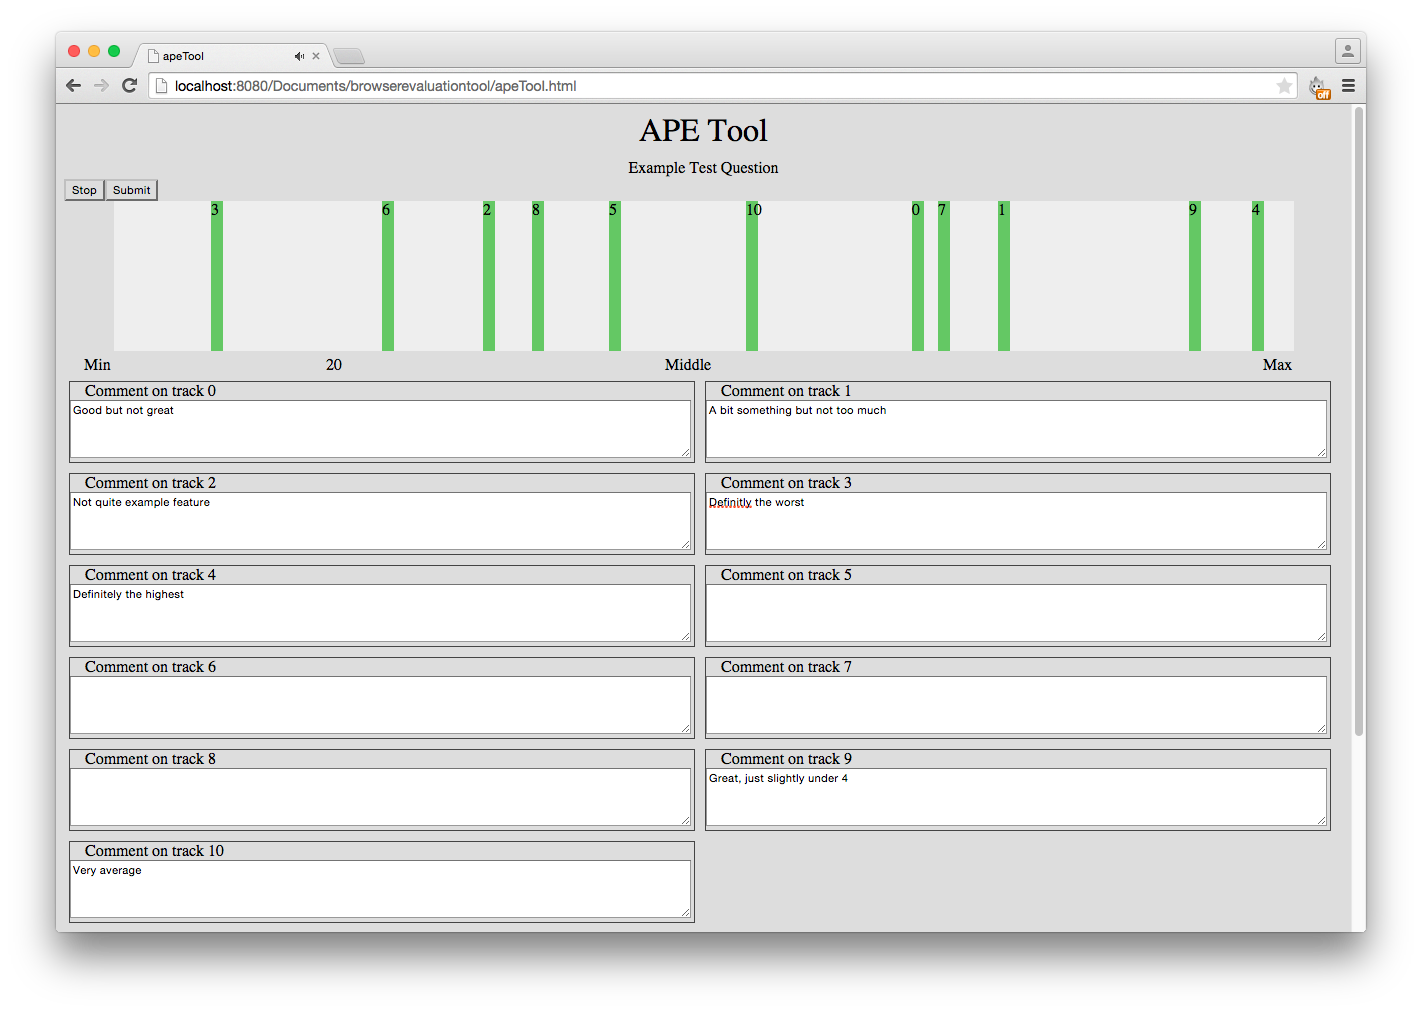
\includegraphics[width=0.9\textwidth]{interface.png}
\caption{Example of interface, with 1 axis and 11 fragments}
\label{fig:interface}
\end{center}
\end{figure*}
[DAVE to make new picture]

[BRECHT to expand]



\section{Architecture}\label{sec:architecture} % or implementation? 

The tool runs entirely inside the browser through the new HTML5 Web Audio API. The API is supported by most major web browsers (with the exception of Internet Explorer) and allows for constructing a chain of audio processing elements to produce a high quality, real time signal process to manipulate audio streams. The API supports multi-channel processing and has an accurate playback timer for precise scheduled playback control. The Web Audio API is controlled through the browser JavaScript and is therefore highly configurable. The Web Audio API processing is all controlled in a separate thread to the main JavaScript thread, meaning there is no blocking due to real time processing. 

The web tool itself is split into several files to operate:
\begin{itemize}
\item \texttt{index.html}: The main index file to load the scripts, this is the file the browser must request to load. %This should be renamed index.html, but will wait until the file is renamed in the repo. 
\item \texttt{core.js}: Contains functions and objects to manage the audio control, audio objects for testing and loading of files. 
\item \texttt{ape.js}: Parses setup files to create the interface as instructed, following the same style chain as the MATLAB APE Tool \cite{deman2014b}.
\end{itemize}

The HTML file loads the \texttt{core.js} file along with a few other ancillary files (such as the jQuery JavaScript extensions)% should we cite jQuery.... https://jquery.com/
, at which point the browser JavaScript begins to execute the on-page instructions, which gives the URL of the test setup XML document (outlined in the next section). \texttt{core.js} parses this document and executes the function in \texttt{ape.js} to build the web page with the given audio files. The reason for separating these two files is to allow for further interface designs (such as MUSHRA \cite{mushra} or A-B tests \cite{bech}) to be used, which would still require the same underlying core functions outlined in \texttt{core.js}, see also Section \ref{sec:interface}.

The \texttt{ape.js} file has several main functions but the most important are \textit{loadInterface(xmlDoc)}, \textit{loadTest(id)}, \textit{pageXMLSave(testId)} and \textit{interfaceXMLSave()}. \textit{loadInterface(xmlDoc)} is called to decode the supplied project document in respect for the interface specified and define any global structures (such as the slider interface). It also identifies the number of pages in the test and randomises the order, if specified to do so. This is the only madatory function in any of the interface JavaScript files as this is called by \texttt{core.js} when the document is ready. The design style is such that \texttt{core.js} cannot 'see' any interface specific functions and therefore cannot assume any are available. Therefore the \textit{loadInterface(xmlDoc)} is very important to setup the entire test environment. It can therefore be assumed that the interface files can `s